\thispagestyle{fancy}

\section{Optische Polarisation und Valenzbandstuktur}
%
\begin{figure}[ht]
    \centering
    \begin{minipage}[t]{0.49\linewidth}
        \centering
        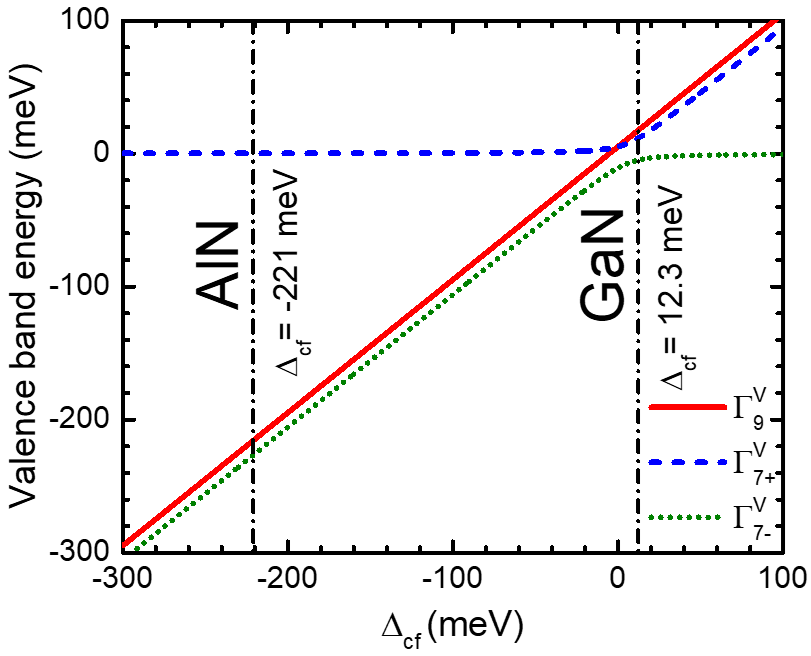
\includegraphics[width=\linewidth]{Bilder/vancebandPlot.png}
        \caption{Die energetische Reihenfolge der Valenzbänder in Abhängigkeit der Kristallfeldaufspaltung. Sichtbar ist der Wechsel der Bandanordnung mit sinkender Kristallfeldaufspaltung und der Effekt des "`anti-crossing"' bei den Bändern gleicher Symmetrie.    }
        \label{fig:auger5k}
    \end{minipage}% <- sonst wird hier ein Leerzeichen eingefügt
    \hfill
    \begin{minipage}[t]{0.49\linewidth}
        \centering
        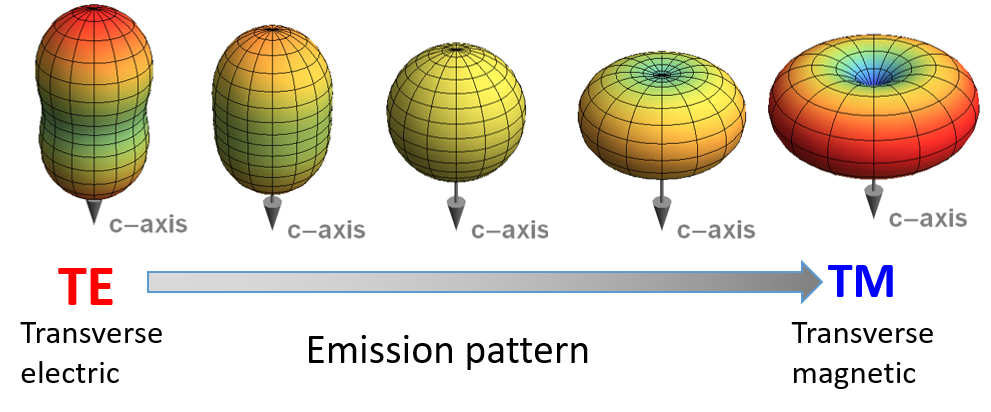
\includegraphics[width=\linewidth]{Bilder/martinTETM.png}
        \caption{Die Grafik zeigt die sich kontinuierlich ändernde Abstrahlcharakteristik in Abhängigkeit der Polarisation von TE- zu TM~\cite{martingut}.  }
        \label{fig:trueiqe}
    \end{minipage}
\end{figure}
\vspace{0.1cm}
\raggedright
Durch die Prozessierung und die Flip-Chip-Montage kann Licht nur durch die untere, unbewachsene Seite des Saphir-Substrates ausgekoppelt werden. Die Art und Weise der Lichtauskopplung hat einen bedeutenden Einfluss auf die Extraktionseffizienz und damit auf die externe Quantenffizienz(EQE). Durch die Geometrie bestimmt, hängt die Extraktionseffizienz maßgeblich vom Emissionsprofil ab, so dass Licht welches senkrecht zur Quantenfilmebene abgestrahlt wird, die höchste Extraktionseffizienz aufweist. 
Um diese zu optimieren, ist es wichtig die Bandstrukturen zu betrachten.
\newline
Die Valenzbandstrukturen von AlN und GaN unterscheiden sich durch die unterschiedliche anordnung der Bänder. Neben dem Leitungsband gibt es ein durch Spin-Bahn-Wechselwirkung und Kristallfeldenergie dreifach aufgespaltenes Valenzband~\cite{doi:10.1063/1.117689}. Sie werden nach ihrer energetischen Lage als A-,B- und C-Band bezeichnet. In AlN hat das A-Band eine $\Gamma^{L}_{7+}$, das B-Band eine $\Gamma^{L}_{9}$ und das C-Band eine $\Gamma^{L}_{7}$ Symmetrie. Bei GaN hingegen gilt folgende Reihgenfolge:  $\Gamma^{L}_{9}$, $\Gamma^{L}_{7+}$, $\Gamma^{L}_{7}$. Die Ursache für den Symmetriewechsel liegt in der großen negativen Kristallfeldenergie von AlN mit einem Wert von $-221meV$ \cite{PhysRevB.87.235209} im Vergleich zur positiven von GaN mit $12,3meV$ ~\cite{PhysRevB.81.155202}. Bei Raumtemperatur wird, nach der Fermi-Dirac-Verteilung, das oberste Band mit der $\Gamma^{L}_{7+}$-Symmetrie, besetzt und aus Zuständen des $p_z$ bestehend, wird transversal magnetisch (TM) polarisiertes Licht emittiert ist. Die strahlende Rekombination findet demnach überwiegend mit Elektronen und Löchern aus dem A-Band mit $\Gamma^{L}_{7+}$-Symmetrie statt.
In GaN ist das oberste Valenzband am $\gamma$-Punkt mit $\Gamma^{L}_{9}$-Symmetrie . Das elektrische Feld des Lichtes ist senkrecht zur c-Kristallachse und wird durch Übergänge ins A- und B- Band erzeugt~\cite{doi:10.1063/1.3574025}, die aus Zuständen des $p_x$-und $p_y$-Orbitals bestehen. Bei strahlender Rekombination von Elektronen mit den Löchern im A- und B-Band entsteht also überwiegend TE-polarisiertes Licht ~\cite{doi:10.1063/1.3574025}. 
TM polarisiertes Licht kann nicht ausgekoppelt werden, da es nur in der x-y- Ebene (parallel zur Quantenfilmebene) emittiert. Daraus resultierend sinkt die Extraktionseffizienz und damit die EQE. Bei $Al_{x}Ga_{1-x}N$ kommt es mit steigendem Aluminiumgehalt zu einer kontinuierlichen Verschiebung der Valenzbänder und es kommt zum sog. "`anti-crossing"' des $\Gamma^{L}_{7+}$ und $\Gamma^{L}_{7-}$ und resultiert in einer Änderung der Oszillatorstärke und damit der Polarisationseigenschaften ~\cite{doi:10.1063/1.4932651}.  Bedeutet, die Lichtemission ändert sich von hauptsächlich TE-polarisiertem Licht zu TM-polarisiertem Licht. Der genaue Aluminiumgehalt, an dem die Valenzbandkreuzung auftritt, ist noch nicht hinreichend bekannt. Theoretische Betrachtungen sagen für unverzerrtes $Al_{x}Ga_{1-x}N$ einen Kreuzungspunkt bei ca. $7\%$ vorher ~\cite{doi:10.1063/1.3675451}. Durch den starken Einfluss von Verzerrungen auf die Energie der  Valenzbandkante, ist die Polarisation abhängig von der wachsenden biaxialen Verzerrung bei steigendem Aluminiumgehalt. So wurde von Kawanishi et al. experimentell der Wechsel bei einem Aluminiumgehalt von "`75\%"' festgestellt ~\cite{doi:10.1063/1.241024}. Noch dazu ist ist die Polarisation bei Mehrfachquantenfilmen(engl. multiple quantum wells, kurz MQW) abhängig vom Ladungsträgereinschluss (engl. quantum confinement). Dieser ist hauptsächlich bestimmt durch die Barrierenhöhe und Barrierendicke. Mit kleiner werdender Barrierendicke, steigt der Grad der Polarisation durch den gesteigerten Einfluss des QCSE ~\cite{PhysRevB.84.035305}. 
\newline
\begin{figure}[ht]
    \centering
    \begin{minipage}[t]{0.49\linewidth}
        \centering
        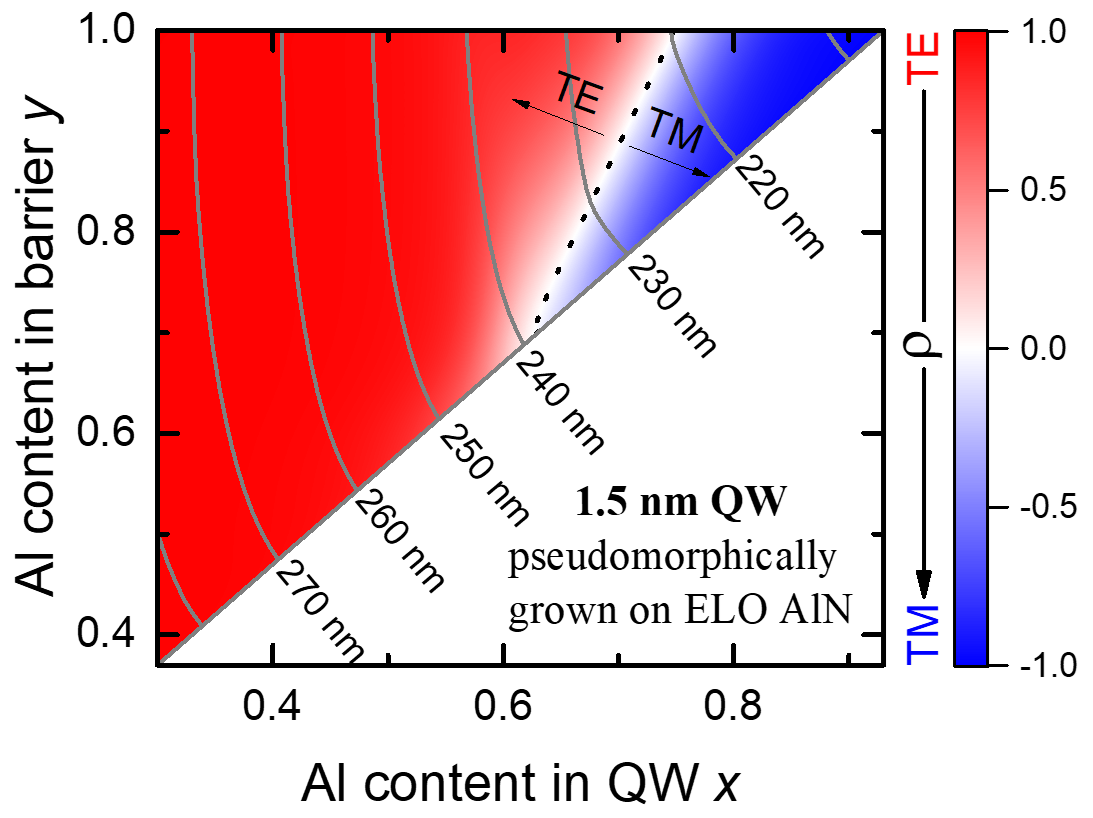
\includegraphics[width=\linewidth]{Bilder/christophPolarisationSimu.png}
        \caption{Simulationsergebnisse des Polarisationsgrades in Abhängigkeit der Aluminiumkonzentration der Barrieren und Quantentöpfe, basierend auf
dem k·p-Modell, für AlGaN-QW mit $1.5nm$-Dicke, die pseudomorph auf ELO-AlN gewachsen wurden. Die gestrichelte Linie zeigt, dass der Wechsel der Polarisation abhängig ist vom Aluminiumanteil in den Barrieren und QWs ~\cite{doi:10.1063/1.4932651} .  }
        \label{fig:simuchr}
    \end{minipage}% <- sonst wird hier ein Leerzeichen eingefügt
    \hfill
    \begin{minipage}[t]{0.49\linewidth}
        \centering
        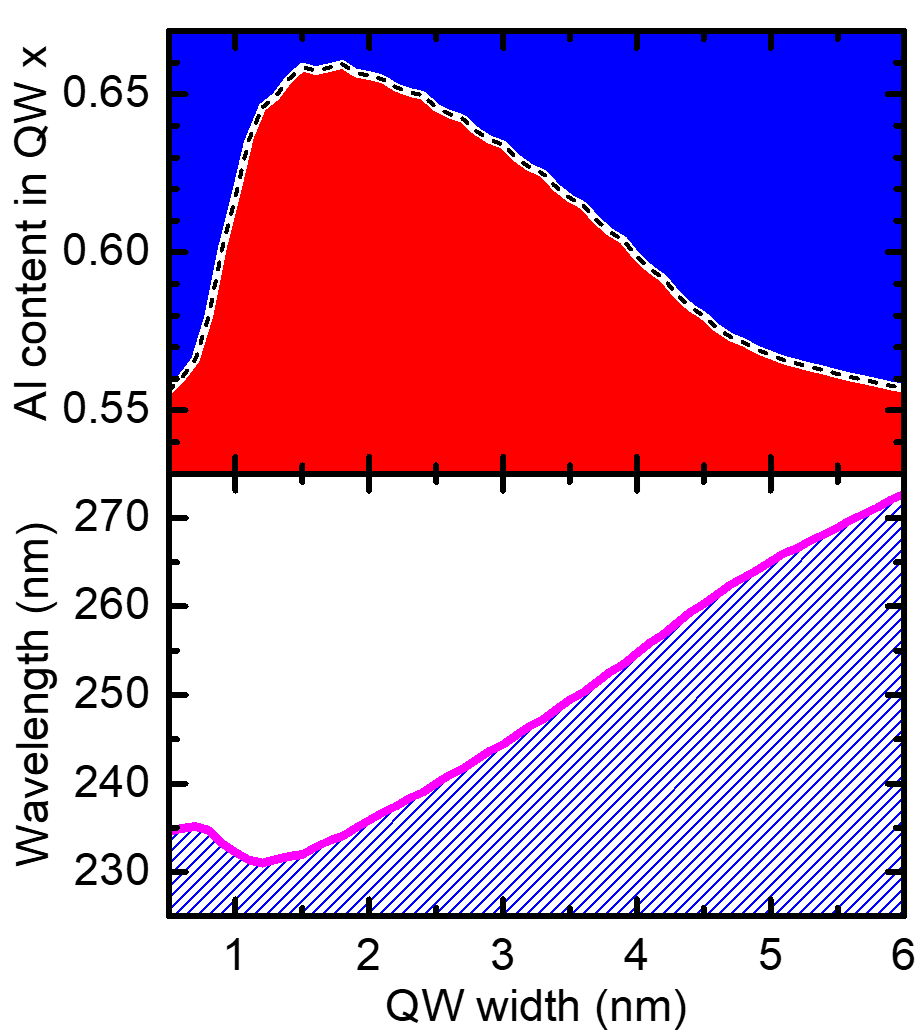
\includegraphics[width=\linewidth]{Bilder/christophPolarisationSimu1.png}
        \caption{ Ergebnisse der Simulation für die Polarisation in Abhängigkeit von der QW-Dicke(Wellenlänge) und dem Al-Gehalt in den QWs ~\cite{doi:10.1063/1.4932651} .  }
        \label{fig:simu1chr}
    \end{minipage}
\end{figure}
\vspace{0.1cm}
\raggedright
Reich et al. untersuchte unter diesem Zusammenhang die optische Polarisation der Emission von UVC-Leuchtdioden(LEDs) auf Basis von (0001) orientierten $Al_{x}Ga_{1-x}N$-MQWs mit Simulationen und Elektrolumineszenzmessungen ~\cite{doi:10.1063/1.4932651}. Dabei stellte er fest, dass mit zunehmendem Aluminium-Gehalt in den QWs die inplanare-Intensität des TE polarisierten Lichtes gegenüber dem des TM polarisierten Lichts abnimmt, was auf eine Neuordnung der Valenzbänder in $Al_{x}Ga_{1-x}N$ zurückzuführen ist. 
Durch Modellrechnungen, basierend auf dem k·p-Modell, wurde das Design der aktiven Zone von AlGaN MQWs optimiert, wodurch eine erhöhte TE-Polarisation und damit eine höhere Extraktionseffizenz für bottom-emitting LEDs im tiefen UV-Spektralbereich ergibt. Unter der Annahme von schmalen Quantentöpfen, Barrieren mit hohem Aluminium-Gehalt und voll verspanntem Wachstum auf AlGaN-Bulk Substraten wurde bei einer Wellenlänge von nur $239 nm$ eine starke TE-polarisierte Emission beobachtet.
Mit Hilfe der Photolumineszenz lässt sich die Polarisation ebenfalls bestimmen, in dem die Polarisation $\rho$ der Photolumineszenzemission aus der Kante einer Probe mit Hilfe der Gleichung 
\begin{equation}
\rho = \frac{ I_{TE} - I_{TM} }{ I_{TE} - I_{TM} } 
\end{equation}
bestimmt wird. Dabei ist $I_{TE}$ die integrierte Intensität der TE-polarisierten und $T_{TM}$ die Intensität der TM-polarisierten Emission. 
 

